\documentclass[version=last,fontsize=13pt]{scrartcl}

\usepackage{pdfpages}
\usepackage{graphicx}

\usepackage{indentfirst}

\usepackage{titlesec}
\usepackage{caption}

\titlespacing*{\section}{0pt}{3ex}{3ex}
\titlespacing*{\subsection}{0pt}{1.5ex}{1.5ex}
\titlespacing*{\subsubsection}{0pt}{1.5ex}{1.5ex}

\usepackage[margin = 0.8in]{geometry}

%my own paragraph for which the text that follows starts on a new line
\newcommand{\myparagraph}[1]{\paragraph{#1}\mbox{}\\}

% dont number sections
% \setcounter{secnumdepth}{0}

\usepackage{wrapfig}
\usepackage{float}

\usepackage{caption}
\usepackage{subcaption}

\usepackage{tabularx}
\usepackage{appendix}

\usepackage{caption}
\usepackage{subcaption}
\usepackage{blindtext}

%settings for providing quotes
\def\signed #1{{\leavevmode\unskip\nobreak\hfil\penalty50\hskip2em
  \hbox{}\nobreak\hfil(#1)%
  \parfillskip=0pt \finalhyphendemerits=0 \endgraf}}

\newsavebox\mybox
\newenvironment{aquote}[1]
  {\savebox\mybox{#1}\begin{quote}}
  {\signed{\usebox\mybox}\end{quote}}

\usepackage{hyperref}


\begin{document}

\begin{titlepage}
	\begin{center}	
		
\includegraphics[width = 5cm,height = 1.5cm]{./imgs/uws_logo.png}\\[5cm]

	{ \huge \bfseries %
		Development and Evaluation of the Usability of a Mobile Web System Designed for Youth Work\\ \Large}

	\vspace{2cm}
	
	\vspace{2cm}			
			

			
		\begin{flushright}
				\large Student:\\
				Marius-Lucian Olariu\\[1cm]
		\end{flushright}
		
	
		\begin{flushleft}
			 \large
				Module coordinator: \\
				Dr. Daune West \\[1cm]
		\end{flushleft}
		
	\vspace{2cm}	
	
		
		\vfill

			{\large {Paisley \\ Word count: ? \\ 2019}}
		\end{center}
\end{titlepage}

\renewcommand{\labelenumi}{\roman{enumi}}

\newpage

\tableofcontents

\newpage


%Read the paper out loud

%FIXME how can you write an abstract as Daune wants before having the full paper written ?!
\section{Abstract}%(5 p - 300w )\\
% Summary of the problem, core problems and how these will be
% addressed. Please include up to 5 key words or phrases at the bottom of the abstract.
% (maximum 300 words – please give word count in document) 

% A pilot study on the development of a Mobile Web system (mobile app and webpage) for YMCA Paisley. Try to provide a mobile-web system with high usability so that the organization wants to adopt it over their old paper based system.\\

Usability is the extent to which a system can be used by specified users to achieve goals with effectiveness. Usability in the context of software leads to user productivity and satisfaction. On the other hand, poor usability leads to underutilization of a software product. While there is a lot of research on web and mobile usability most of them analyze software that is already developed and test usability guidelines or propose new ones. The author has managed to find only one study where a mobile website was developed and developed for a practical setting, namely for library services.  In this pilot study the author developed a website and a mobile application designed for the youth work of YMCA Pailsey. The  system used by YMCA Paisley relies on paper forms to collect information about volunteering sessions, schedule volunteering/mentorship sessions and receive feedback. The mobile-web system was compared against the "traditional" system used by YMCA Pailsey from their usability perspective. The methodology used a structured interview for collecting data, namely, interviews were taken to the YMCA volunteers before and after the mobile-web system was deployed. The results of this research enrich the usability knowledge about mobile-web systems. Moreover, YMCA Paisley gained valuable insights regarding their youth work and if an investment in such a system should be made. The limitation to this study was time, namely only 15 weeks. Further research can analyze if the finding in this study hold for other organizations of YMCA Scotland.\\

Key words: \textbf{usability evaluation, usability, website, mobile application}

\section{Aims}

%\section{Aims}(5 p - 125w )\\
% General statements on intent and direction of the research
\indent
The main aim of this work is to develop a prototype webpage and a mobile application for the youth work of YMCA Paisley and to compare it from the usability perspective with the current system used by the organization. The current system  relies on paper forms to collect information about each volunteering session which have to be analyzed by the organization's manager.  In this work the term mobile-web system is going to describe the two software artefacts (webpage and mobile application). The mobile-web system would provide valuable insights for the organization  regarding their activity. Moreover, once the study is finished the organisation can decide if it is worth to invest in the development of such a system  or not. 
%YMCA Pailsey is a nonprofit organization thus it needs to do a thourugh assesment regarding any investition.

\section{Objectives}%(10 p - 250w)\\
% A list of clear, measurable statements of intended outcomes. i.e. What you are going to do in order to answer the question in the title and how you are going to do this (in relative detail) 
A literature research should be performed to see if there are similar projects, how have they been developed and evaluated. The next step is to have one or two meetings with the users (manager and volunteers alike) of the mobile-web system in order to derive a  set of software requirements. Once this is done a project document should be written containing the following headings: description of project, system requirements, system specifications and software design methods. This document should be made available to all the parts invovled (developers, volunteers, manager) so that they can provide additional input. Apart from development, an evaluation is necessary which is split in two parts: technical  and non-technical. To perform the technical evaluation of the software the developers have to write unit tests. The non-technical evaluation uses a structured interview regarding usability of the system used in the youth activity of YMCA Paisley. Once the structured interview is devised, the researcher can interview the manager and the volunteers to obtain initial data. The next step is to deploy the mobile-web system for 1 - 2 weeks and do the interview again. At this point the data obatained by the researcher can be evaluated and conclusions drawn.


\section{Justification} %(5 p - 125 w)\\
 % Rationale for the research showing gaps in current knowledge
% and how the results of the research might be used.
% (Aims, Objectives, Justification – about 1 page) (5 marks)
	\indent
	The author believes that there is a gap in the literature for  research that develops  and evaluates a mobile-web system and how this can improve (or not) the activity of an organization from the perspective of its usability. To motivate aforementioned statement the author is going to enumerate the research analyzed in the literature review. Gündüz and Pathan (2012) study the usability problems of mobile flight booking apps and provide usability guidelines to help developers to create mobile flight booking apps. Shitkova et al (2016) studied and compiled a large number of usability guidelines published in literature (2003 - 2013) and applied them in the developement and evaluation of a mobile app and a mobile website. Ismailova (2017) identified the usability problems of government websites of Kyrgyz Republic and the fact that low priority was given to usability in government websites development. ChanLin and Hung (2016) developed a mobile website for a library with usability in mind and managed to provide better search facilities compared to the desktop variant of the website. The results of this research enrich the usability knowledge about mobile-web systems. Apart from the research underpining of this project it is worth to mention that the author is volunteering with YMCA Paisley and this research represents a good opportunity to put in practice the knowledge acquired during his Mobile Web Development master studies.\\



\section{Review of the literature } %(20p - 1700w - 2000w)\\
	% Review of Literature: History of problem with key sources with critical appraisal of contributions.
% (guidance - no more than 2000 words – please give word count in document)
% (20 marks)

%peer review  
%talk about weaknesses (suggest ways to improve) and strengths
%table and graphs signposted
%mention in your work the weaknesses and future work

%FIXME should I remove the subsections?
\subsection{Filtering conditions for finding relevant research}
	The author has tried to find literature that contains  mobile and/or webpage development and is related to usability. One of the first search queries used in Google Scholar (n.d.) was "mobile booking" and on the second page of the results was found the research by Gündüz and Pathan (2012), other works matching the search query have been read but not mentioned as part of literature review due to poor quality (Karthick, S. and Velmurugan, 2012; Abdullah and Kadhim, 2016). Details for finding other research papers are omitted (to save space) and just the queries used are enumerated:  "mobile-web usability", "usability guidelines mobile", "cross-platform development".

\subsection{Usability for Mobile-Web}

\indent
%introduction and mobile usability
%write about how you found the literature
	The world of phones and computing changed in 2007 when the first iPhone was released due to the fact that this phone allows users to access Internet, has a touchscreen interface and is essentially a small computer that fits in a pocket. The term \textit{smartphone} is used to describe such a device. At the time of writing of this work (2019) there are about 2.71 billion smartphone users around the world and the number is expected to increase in the future (Number of smartphone users worldwide 2014-2020, n.d.). Such a large pool of users drives big companies to invest in their mobile applications and their websites in order to provide better customer experience (Vagrani, Kumar and Ilavarasan, 2017).\\ 
	All major airlines companies nowadays offer booking facilities both through their website and mobile app. Apart from the security to protect user data usability is another important characteristic in this industry since it leads to fast flight booking, thus generates revenue. Nielsen (2012) even suggests that 10\% of  the project's budget should be invested in usability. While the purpose of this work is not related to any e-commerce industry, it is still worth to analyze how these booking systems are designed to increase usability in  order to develop a better mobile-web system. One of the crucial factors for using a mobile-web app from the perspective of the users is \textit{usability} and \textit{user experience}. However, there are different opinions in literature to what these terms mean. To eliminate any confusion that might arise their definitions from ISO 9241-210:2010 (2010) are provided below.

\begin{aquote}{ISO 9241-210:2010, 2010, non-paginated}
	\textit{User Experience - person's perceptions and responses resulting from the use and/or anticipated use of a product, system or service.}	
\end{aquote}

\begin{aquote}{ISO 9241-210:2010, 2010, non-paginated}
	\textit{Usability -
extent to which a system, product or service can be used by specified users to achieve specified goals with effectiveness, efficiency and satisfaction in a specified context of use}	
\end{aquote}

The user experience and usability have common characteristics, however, the former is harder to evaluate (McNamara and Kirakowski, 2005).
The design of a webpage is not affected by many variables as it is the case for a mobile app. When designing a mobile app one has to take into account that the user might be on the move, a variable screen size, limited processing power, user's attention interruptions or poor network connection (Oulasvirta et al, 2005). Following their study on usability for a mobile flight booking app Gündüz and Pathan (2012) have identified  usability challenges that are going to be briefly detailed. Icons help in saving screen space and aid in completion of tasks, however, \textit{the wrong choice of icons} leads to confusion, it is suggested to use the same icons on web and mobile app to have consistency. Next, the mobile interface needs  to have \textit{a smaller number of steps} compared to the web app to achieve a task (e.g. search for flights) due to the fact that network interruptions might occur. Subsequently, the user inputs in a mobile app should be located towards the bottom of the screen to \textit{favor single hand use of the device}. Lastly,  there should not be presented a lot of information at once (cognitive overload) and the most important bits should be highlighted (e.g. departure and return date for a flight).\\
\indent
	Another study by Shitkova et al. (2015) focused on finding usability guidelines for mobile applications and mobile websites tested in empirical settings and published in a large time frame, between 2003 and to 2013. In total there were identified 39 usability guidelines (from 127 papers) which were structured in the following 5 categories: i) Layout, ii) Navigation, iii) Design, iv) Content and v) Performance. To demonstrate the aplicability of the usability guidelines found the researchers developed a mobile app and a mobile website. While the author considers most of the presented guidelines to be useuful, there is one, \textit{"G3) ...avoid using tabs"} which is not necessary valid because the \textit{Tab Bar Design} is widely used in succesful apps (e.g. Coursera, edX, Facebook) and sugested by famous organizations as good practice (Nielsen Norman Group, 2015).  Similar to the findings of Gündüz and Pathan (2012), in this research it was higlighted the guideline \textit{of having a consistent user interface between the mobile website and the mobile app}.\\

%web usability
\indent
Web Usability guidelines have been around from 1990s and nowadays there are well established publications regarding this topic (Nielsen Norman Group, n.d; Shneiderman and Leavitt, 2006). We can say that Web Usability is a mature field now after almost 30 years of research. Websites within e-commerce sector pay a special interest in usability since it stimulates online purchases (Venkatesh and Agarwal, 2006). Another sector where website usability is crucial is represented by government's websites because the information posted there is of interest to the whole population of a country. One expects that governements would make a priority for their websites to be usable, however, that is not always the case. For instance, an analysis of Kyrgyz Republic 60 government websites revealed that they have an usability error rate of 69.38\% (Ismailova, 2017). The usability tests performed in the research of Ismailova (2017) were automated and performed with various software products that checked for broken links withing the tested website, upload speed of main page  and the page size of the main page. This research found that low priority was given to usability when the Kyrgyz Republic websites were developed.\\
\indent
	Apart from providing a usable website for the desktop view for this project it is worth to analyze what things matter for providing a usable website for the mobile  as well. Mobile websites and apps are being extensively used nowadays in providing library services and they encourage collaboration and knowledge exchange between learners (Hopkins et al., 2015). To increase website usability one can develop different versions of the  website for different categories of screen resolution. Therefore, when the user accesses the website from mobile the mobile variant is sent to the browser. Developers also need to consider removing some parts of the mobile website compared to the desktop variant due to the limited screen size of the mobile devices. As was suggested for mobile apps regarding flight booking (Gündüz and Pathan, 2012) there is a need to \textit{reduce the number of total steps} required to access information in a mobile website (Murray, 2010).\\
ChanLin and Hung (2016) compared the variants of a website (desktop and mobile) for a library from the usability perspective of the two. The desktop variant of library website was already in use, thus, the authors developed the mobile website. To evaluate the usability of the websites the authors conducted a test on 50 users (students) that had to  complete library search tasks on the mobile and desktop websites. For each user was recorded the number of search tasks completed, time required and accuracy of the results provided. The data showed that the users managed to finish more search tasks in less time on the mobile website. The authors also used an online survey with Likert questions (scale 1-5) with 366 respondeds and the outcome was positive towards the mobile website with a mean higher than 4 for each question.

	\subsection{Cross-platform development approach}
	%mby add a bit about the web
	The mobile app needs to be developed for both major mobile \textbf{o}perating \textbf{s}ystems (OS), namely, Android and iOS. This implies  to write the code for the application twice, once in Java  for Android and once in Swift for iOS, this approach is known as native app development. While this is the ideal way to obtain app performance it is not feasible given the total time allowed for a MSc project. Therefore, to save time one can use a \textbf{c}ross-\textbf{p}latform \textbf{t}ool (CPT) where the codebase is written just once and the CPT generates an applcation for multiple mobile OSs. However, there are many CPTs available and it is hard to choose one that best fits a project without prior research. To get an ideea of how many options are available, for instance, in an industry report by SlashData (2012) there were discussed more than 100 CPTs. The same report (SlashData, 2012) higlights that developers' satisfaction regarding CPTs has been low, however, the author believes that some CPTs are now mature and better suited for development. \\
	\indent
	There are 5 types of CPTs: i) app factories, ii) source code translators, iii) JavaScript frameworks, iv) runtimes and v) Web-to-Native. The app factories target non-developers and help them to create a basic app by using drag-and-drop visual elements (the process is similar to solving a puzzle). JavaScript frameworks allows web developers to develop mobile apps using client-side technologies (HTML, CSS and JavaScript) the resulting mobile app is basically a webpage for mobile that can be accessed through a mobile browser. Web-to-Native are similiar to JavaScript frameworks in terms of development technologies just that this CPT packs the mobile website into a standalone mobile app that can be installed on the devices. 
	%Runtime CPTs have their own language for writing the app code which is directly complied to executable code for a mobile OS. 
	Runtime CPTs allow developers to write the non-native app using a language like Java and provide a special runtime for executing it for each mobile OS; basically,  the native app is comprised of the non-native part and the runtime that executes it.  
	Source code translators CPTs allow one to write the app code in a specific language which later is translated to the equivalent code for a specific mobile OS (e.g. Java/Swift) which in turn is compiled to executable code.\\
	\indent
	A complex analysis of 10  CPTs was done by Willocx, Vossaert and Naessens (2016) resulting in a series of guidelines for picking a CPT. Apps developed with JavaScript frameworks stress more the CPU and consume more memory than native apps, however, their performance is comparable to their native counterparts. The size of the app installer and the memory consumption is increased when using runtime CPTs compared to a native app. The best choice from a technical perspective it seems \textit{source code translators} that provide performances comparable with the native approach. Apart from these technical considerations, there are some non-technical considerations that can help in decision process: existing infrastructure (Webpages can be directly converted to mobile using JavaScript CPTs), skills of developer (one can pick a CPT that uses technologies he knows), flexibility (some CPTs offer better support to access OS specific features) and type of application (some CPTs are better for developing game apps). Given the above guidelines the author is going to use Flutter (n.d.), a CPT developed by Google, which is a source code translator according to the above classification because the performance of the app will be close to the native counterpart.

	%it is reasonable to look to use a cross platform development tool. To analyse which options are the best I read a paper

\section{Methodology}%(25 p - 1000w)\\
	 % Explanation and justification of approach and methodology proposed. This section should explain the nature of the data you expect to collect; who will be involved and how you will collect it? Clear signposting of selection process of organisations/groups/individuals involved in the study should be explained. Identification and brief discussion of any analytical tools to be used; Identification of any ethical issues.
% (guidance – no more than 1000 words – please give word count in document) 

%likeart-type scale

% talk about the whole development process
\subsection{Software Development}
 	As was mentioned before in this research proposal the software system is comprised by two components, namely, a webpage and a mobile application for the two major mobile OSs (iOS and Android). These two software products need to share a common database where all the data is stored. Data is generated by the volunteers using the mobile app and can be viewed by the manager and edited.\\
	\indent
	%web
	When it comes to webpage development and Web Development in general there are many technologies that one can use for both client-side development and server-side development. The look and feel of the webpage does not need to have complex visual features, thus, its development can be done using HTML5, CSS3, JavaScript and AJAX. There are many server-side development languages that one can use like PHP, C\# (ASP.NET) or Python frameworks (Django, Flask). However, the author is going to use PHP due to the following reasons: past development experience with the language, it has a large community around it (Cass, 2018), can be embedded in HTML code and the stack \textbf{L}inux-\textbf{A}pache-\textbf{M}ySQL-\textbf{P}HP (LAMP stack)is free. Due to the fact that the webpage will contain a login feature and use a database extra security measures are needed. Namely, the login input needs to be sanitized to protect the webpage agains all kind of attacks simillar to  SQL Injection.\\ 
	\indent
	%database
	Although MySQL database and PHP are often used together when developing webpages, for this project the author is going to use \textbf{F}irebase \textbf{R}ealtime \textbf{D}atabase (FRD). MySQL is a relational database which stores data in tables that have relationships and constraints among them, however, not all types of data can be easily structured in such a database type. Therefore we have document-oriented databases like FRD which work better for storing 'unstructured' data which is going to be the case for this project. Another reason to use FRD is the fact it integrates very well with object oriented programming languages that are going to be used like PHP and Dart (for the mobile development).\\ 
	\indent
	%mobile
	The best approach to develop the mobile apps would be the native one, namely, to write the iOS app in Swift with Xcode and the Android one inJava with Android Studio. However, this approach is time consuming, a macOS machine for iOS development is needed and the author is not very familliar with Swift progamming. Therefore, a cross-platform approach will be put in practice, which means that the codebase for the mobile apps is written only once and the two apps are generated by a CPT. As was presented in the literature review there are many CPT to choose from but for this project Flutter (n.d.) is going to be used. To mention but a few reasons to use Flutter: hot reload (allows code to be injected on a running app; improves development time), the generated apps use native UI elements, open-source, good documentation materials and the possibility to use a familliar \textbf{I}ntegrated \textbf{D}evelopment \textbf{E}nvironment (IDE) like Android Studio. However, the iOS application cannot be published on AppStore due to the fact that now Apple accepts only applications that are written 100\% native in Swift.\\
	%git
	\indent
	In order to keep track of all the code files there is going to  be used a version control website, GitHub (n.d.). The whole codebase is going to be contained in a repository with different submodules that can be updated independently. 
	

	%git
% talk about data collection, about manager and volunteers/staff (instructed by the manager to take part in it), how you analyse data
\subsection{Data collection and evaluation}
	In order to evaluate the usability of the mobile-web system compared to the current system ("paper forms") used by YMCA Paisley a structured interview is going to be used. In total, a number of 6 persons are going to be interviewed, namely, the YMCA Pailsey manager and 5 other volunteers. The YMCA Paisley has around 25 volunteers, therefore, more than one fifth of the organization is going to be interviewed. Nielsen (2000) argues that for usability testing  only 5 users are enough. The volunteers are selected based on how long they have been volunteering within the organization, from less experienced to more experienced ones. There are two methods suitable to conduct the interviews, namely, \textit{face-to-face} and via \textit{telephone call}. %describe them if you want to add more words. FIXME modify the weeks when the interview takes place once you adjust the table to 15 week. 
	The author is going to use the \textit{face-to-face} approach because it offers also non-verbal information regarding what the interviewees think about the developed mobile-web system and the current system.  The author is going to organize two meetings to conduct the interviews, one in week 6 and one in week 12 (see Figure~\ref{gC}). There are no monetary costs involved for the volunteers or the author to come to this meetings because they can be held before/after the weekly organizaton's meeting. %To each answer received to the interviews question a value is going to be assigned, range 1-10.

% talk about ethics
\subsection{Ethical and practical considerations}
	Before a young person starts a YMCA mentorship their parents/tutors must agree that YMCA processes and stores data regarding the young person. Due to the fact that such a mobile-web system uploads the young person's data on the Internet it must be very secure and has to comply with tough government regulations. However, because this is a plot study all the data that is going to be uploaded in the time the system is up is going to be spurious. In this way, there are no legal implications for the organization or for the author if somehow the mobile-web app gets hacked. 

\pagebreak
\section{Work plan}%(10p - )\\
%do I need to write smth here or the gantt chart is enough?
To present the stages and their time duration please see the following Gantt diagram.

	\begin{figure}[H]

		%modify this to reflect the 15 weeks of the MSc project
		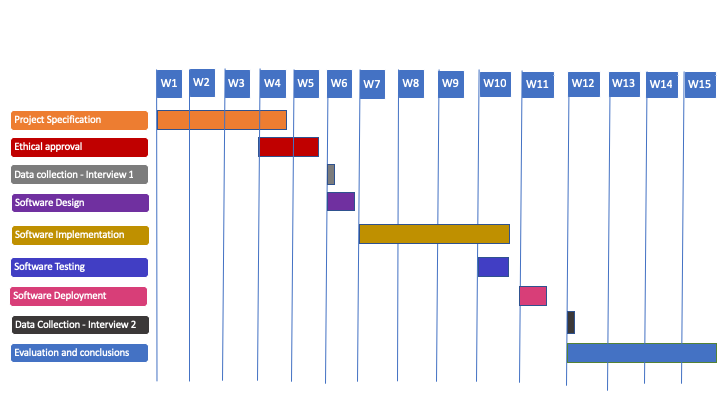
\includegraphics[scale = 0.5]{./imgs/ganttChart}
		\caption{All the activities that need to be undertaken to finish the project}
		\label{gC}

	\end{figure}

\pagebreak

%FIXME remove unused references
%FIXME check they are in alphabetical order
\section*{References}
Abdullah, M.N. and Kadhim, E.H. (2016) Airline mobile reservation development.  \underline{International Advanced Research Journal in Science, Engineering and Technology} [Online]  pp.1-3. Available: https://iarjset.com/recent-issue-october-2016/ [Accessed: 6 April 2019]\\

% Burmistrov, I. (2009) Mobile air ticket booking.  \underline{European Conference on Cognitive} \underline{Ergonomics: Designing beyond the Product}\underline{---Understanding Activity and User}\\ \underline{Experience in Ubiquitous Environments} Article 11 Helsinki: VTT Technical Research Centre of Finland.\\

Cass, S. (2018) The 2018 Top Programming Languages.  \underline{IEEE Spectrum} (July 2018) [Online] Available: https://bit.ly/2AquJBT [Accessed: 10 April 2019]\\

ChanLin, L.J. and Hung, W.H. (2016) Usability and evaluation of a library mobile web site. \underline{The Electronic Library} Vol. 34(4), pp.636-650.\\

\underline{Flutter} (n.d.) [Online] Available: https://flutter.dev [Accessed 5 April 2019]\\

\underline{GitHub} (n.d.) [Online] Available: https://github.com/ [Accessed 6 April 2019]\\

\underline{Google Scholar} (n.d.) [Online] Available: https://scholar.google.co.uk/ [Accessed 3 April 2019]\\

Gündüz, F. and Pathan, A.S.K., (2012) Usability improvements for touch-screen mobile flight booking application: A case study.  \underline{International Conference on Advanced } \underline{Computer Science Applications and Technologies}  pp. 49-54. Kuala Lumpur: IEEE.\\

Hopkins, P., Hare, J., Donaghey, J. and Abbott, W. (2015) Geo, audio, video, photo: how digital convergence in mobile devices facilitates participatory culture in libraries. \underline{Australian Library Journal} Vol. 64(1), pp. 11-22.\\

\underline{ISO 9241-210:2010} (2010) [Online] Available: https://bit.ly/1j1dMhv [Accessed: 3 April 2019].\\

Ismailova, R. (2017) Web site accessibility, usability and security: a survey of government web sites in Kyrgyz Republic. \underline{Universal Access in the Information Society} Vol. 16(1), pp. 257-264. \\

Karthick, S. and Velmurugan, A. (2012) Android suburban railway ticketing with GPS as ticket checker.  \underline{IEEE International Conference on Advanced Communication }\\ \underline{Control and Computing Technologies (ICACCCT)} pp. 63-66  s.l.: IEEE\\

McNamara, N. and Kirakowski, J., (2005)  Defining usability: quality of use or quality of experience?  \underline{IPCC 2005. Proceedings. International Professional Communication} \underline{Conference} pp. 200-204. Limerick: IEEE.\\

Murray, L. (2010) Libraries like to move it, move it.  \underline{Reference Services Review} Vol. 38(2), pp. 233-249.\\

Nielsen, J. (2000) \underline{Why You Only Need to Test with 5 Users} [Online] Available:\\  https://bit.ly/1IbBiWV [Accessed: 10 April 2019]\\

Nielsen, J. (2012) \underline{Usability 101: Introduction to Usability} [Online] Available:\\ https://bit.ly/1OOHO8T [Accessed: 7 April 2019]\\

Nielsen Norman Group (n.d.) \underline{Usability Guidelines for Accessible Web Design} [Online] Available:  https://bit.ly/2s63gO9 [Accessed: 7 April 2019]\\

Nielsen Norman Group (2015) \underline{Basic Patterns for Mobile Navigation} [Online] Available: https://bit.ly/1RpvkVo [Accessed 7 Apr 2019]\\

\underline{Number of smartphone users worldwide 2014-2020} (n.d.) [Online]  Available:\\ https://bit.ly/2dk8wHh [Accessed: 3 April 2019].\\

Oulasvirta, A., Tamminen, S., Roto, V. and Kuorelahti, J., (2005) Interaction in 4-second bursts: the fragmented nature of attentional resources in mobile HCI. \\

\underline{ Proceedings of the SIGCHI conference on Human factors in computing systems} pp. 919-928. New York: ACM. \\

Shitkova, M., Holler, J., Heide, T., Clever, N. and Becker, J. (2015)  Towards Usability Guidelines for Mobile Websites and Applications.  \underline{Wirtschaftsinformatik} pp. 1603-1617 \\

Shneiderman, B. and Leavitt, M. (2006) \underline{Research-based web design \& usability}\\ \underline{guidelines} Washington: Department of Health and Human Services\\

SlashData (2012) \underline{Vision mobile cross-platform developer tools 2012}  [Online] Available: https://bit.ly/2GhaYMC [Accessed: 5 April 2019].\\

Vagrani, A., Kumar, N. and Ilavarasan, P.V., (2017) Decline in Mobile Application Life Cycle. \underline{Procedia computer science}. vol. 122, pp. 957-964. [Online] Article in Press. Available: https://doi.org/10.1016/j.procs.2017.11.460 [Accessed 3 April 2019].\\

Venkatesh, V. and Agarwal, R. (2006) Turning visitors into customers: A usability-centric perspective on purchase behavior in electronic channels. \underline{Management Science} Vol. 52(3),  pp. 367-382.\\

Willocx, M., Vossaert, J. and Naessens, V. (2016) Comparing performance parameters of mobile app development strategies.  \underline{2016 IEEE/ACM International Conference on} \underline{Mobile Software Engineering and Systems (MOBILESoft)} pp. 38-47.  Austin: IEEE.\\

\end{document}

